%!TeX root = thesis-main.tex
\chapter{\introductionname}\label{chap:introduction}\mtcaddchapter
\minitoc% Creating an actual minitoc
\begin{refsection}
\section{Research Background and Context}
Computation is \textit{everywhere}. 
 This statement is not just a catchy phrase but a reflection of our current reality, 
 shaped by the accelerated development of information technology. 
 Indeed, computation has been seamlessly integrated into our everyday lives, 
 so much so that it often goes unnoticed. 
%
Its \emph{ubiquitous} presence transcends traditional boundaries, 
 not just in professional settings but also in our homes, transportation systems, 
 and even our bodies, as evidenced by \emph{wearable} technologies. 
% 
This phenomenon is most evident in the explosion of \ac{iot} devices. 
 According to recent statistics~\footnote{\url{https://www.statista.com/statistics/1183457/iot-connected-devices-worldwide/}}, 
 there are currently over 15 billion IoT devices globally, 
 and this number is expected to surpass 30 billion by the year 2030.

The widespread adoption of computational technologies has ushered in a transformative phase for the IT landscape, 
 starting from the \emph{edge} of the network where connected devices are becoming more sophisticated and efficient. 
 These edge devices are not merely passive data collectors but are now capable of \emph{localized} computation  (thus \emph{cyber-physical}), storage, and analytics. 
Moving towards the core, 
 \emph{cloud} infrastructures are also undergoing significant metamorphosis. 
 Traditional centralized data centres are evolving into a more distributed,
 decentralized, and dynamic architecture to meet the ever-changing demands of users and applications.

In this light, the term \emph{edge-cloud continuum} aptly encapsulates the current IT landscape. 
 It symbolizes a \emph{fluid} environment where the edge and the cloud are not isolated silos but exist as two poles on a spectrum. 
 Between these poles lies a multitude of intermediate layers, 
 comprising \emph{fog computing}, micro data centres, and hybrid cloud solutions, among others. 

This fluid computational landscape is endorsed by contemporary theories like  ubiquitous~\cite{ubiquitous}, pervasive
 ~\cite{DBLP:journals/computer/SahaM03}, everyware~\cite{greenfield2010everyware}, and collective~\cite{DBLP:journals/computer/Abowd16} computing.
%
These paradigms collectively herald an era where computation 
 is not confined to specific devices but emerges as an integrated capability across a vast, 
 interconnected ecosystem in which a vast array of simple devices interact in a decentralized fashion, 
 harnessing their collective might to accomplish intricate tasks often far beyond the capability of individual units. 
%
Drawing from natural systems, 
 it is striking how these intricate computational networks mimic the complex collective behaviours seen in nature. 
 For example, certain social insects, like ants and bees, display remarkable examples of resilient, effective, and efficient self-organizing systems. 
 Such natural phenomena serve as powerful metaphors for understanding and conceptualizing the self-organizing propensities within computational systems.
 
These observations have culminated in the formulation of the concept of \acp{cpsw}, 
 an ensemble of \emph{heterogeneous} computational entities deeply integrated with the physical world. Unlike monolithic systems, \acp{cpsw} leverages diversity—both in terms of device capabilities and functionalities—to achieve collective objectives. 
 This heterogeneous nature enriches the system's adaptability, robustness, and overall performance, thereby enabling it to solve problems in a more nuanced manner.
%
Instances of \acp{cpsw} are becoming increasingly prevalent and varied, 
 seen not only in the realm of swarm robotics but also in human crowd dynamics and in the burgeoning field of IoT devices. 
 In each of these cases, the core principles remain consistent: the employment of self-organizing mechanisms to achieve collective goals in an efficient, resilient, and \emph{adaptable} manner.

\section{Overview and Contribution}
Addressing the engineering challenges of \ac{cpsw} requires innovative approaches, 
 as traditional device-centric and bottom-up methodologies fall short. 
The complexities involved in these swarms stem from a myriad of factors, 
 including the nuanced interaction between local and global dynamics, 
 the intricacies associated with distributed control systems, 
 the evolving landscape of IT architectures, and significant scalability considerations.
%
Given these multifaceted challenges, 
 this thesis introduces a comprehensive \emph{language-based} approach that incorporates robust models, 
 cutting-edge techniques, and pioneering algorithms. 
 The objective is to streamline the design and deployment of self-organizing behaviours in \acp{cpsw} that are both \emph{predictable} and \emph{adaptable}. 
This is achieved by integrating established manual design methodologies, namely aggregate computing~\cite{aggregatecomputing}, 
 with cutting-edge advances in machine learning, such as \ac{marl}~\cite{busoniu2008comprehensive}. 
%
This \emph{hybrid} approach aims to harness the strengths of both paradigms to create a more robust, efficient, and scalable \ac{cpsw} framework.

The research underpinning this work draws from a wide array of interdisciplinary fields, 
 such as swarm robotics~\cite{brambilla2013swarm}, multi-agent systems~\cite{dorri2018multi}, collective adaptive systems~\cite{ferscha2015collective}, field-based coordination~\cite{mamei2006field}, and multi-agent reinforcement learning. 
By synthesizing insights from these diverse domains, 
 the proposed approach aims to offer a holistic solution for the effective engineering and deployment of \acf{cpsw}.
\subsection*{Problem statement}
The current state-of-the-art solutions in both automatic and manual design are limited in handling the complexities arising from the collective intelligence of \ac{cpsw}. 
 While the former may offer gold-standard solutions through a ``learn-by-doing'' approach, 
 they often struggle to generalize across different scenarios. 
 On the other hand, manual solutions may excel in modularity and declarative design but frequently fall short when it comes to managing complex environmental conditions.
\paragraph*{Research questions}
\begin{itemize}
    \item[\textbf{RQ1}:] What is the optimal model for engineering such applications?
    \item[\textbf{RQ2}:] Does a hybrid approach that combines both automatic and manual design offer any advantages? 
    \item[\textbf{RQ3}:] Are there specific requirements for \ac{cpsw} that differentiate them from other large-scale distributed systems?
    \item[\textbf{RQ4}:] how does the engineering of these applications influence the design process for collective controllers?
\end{itemize}

\subsection*{Contributions}

The thesis contributes (summarized in \Cref{fig:contributions}) to an area called ``language-based engineering,'' where models, algorithms, machine learning solutions, and tools are constructed around a specific programming language within a given context.
In the realm of software engineering, 
 a language-based approach is fundamentally concerned with describing tools, models, and applications using high-level abstractions provided by a specific programming language. 
 One of the unique attributes of this methodology is its domain-specific nature. 
 In essence, it starts by establishing a reference framework, 
 constructs the necessary abstractions to articulate the possible behaviours of a given application, 
 and then employs a Domain-Specific Language (DSL) to formulate solutions.
%
For the purpose of this dissertation, 
 we have selected \ac{cpsw} as our broad reference class of systems. 
 We observed that the existing paradigm of aggregate computing (AC) 
 is particularly well-suited for describing emergent behaviours straightforwardly and effectively. This suitability arises from the top-down nature of AC and its capacity to express self-organizing emergent behaviours.
%
Building on this foundation, 
 we adopted a layered approach to bridge the gaps between aggregate computing and the broader domain of reference. 
 In this endeavour, 
 we initially sought to identify the \emph{facets} to target in order to close this gap, 
 which can be broadly categorized into \emph{platform}, \emph{language}, and \emph{design patterns}. 
 At the platform level, 
 we considered all aspects related to executing and deploying a program written in the reference language. 
 At the language level, we aimed to determine if any unique features are particularly relevant to \ac{cpsw}. 
 These choices could also be influenced by platform-specific factors, 
 such as the optimal way to run a certain program. 
 Finally, above the language layer, 
 we attempted to identify a set of design patterns, encompassing algorithms, APIs, and libraries, 
 that could be effective in describing collective behaviours in CPWS.
 Then, we have utilized both standard engineering techniques--
 proposing new programming models specifically tailored for the intricacies of CPWS and developing APIs that bring programmers closer to this complex landscape--
 as well as \emph{unconventional} methods. 
 The latter, which we term as ``hybrid,'' 
 is based on the facets identified above and the engineering approaches proposed
 integrating Artificial Intelligence techniques 
 to either enhance certain aspects of the existing paradigm or improve the learning process itself.
% 
Lastly, this research offers a modern perspective on software engineering, 
 made increasingly relevant by the advent of large language models like GPT~\cite{floridi2020gpt} and LLaMa~\cite{touvron2023llama}. 
 The role of such AI models in assisting and guiding the software development process can no longer be ignored, 
 signalling a new era where human programmers are augmented by intelligent systems capable of facilitating more effective development strategies.
Specifically, our contributions toward a hybrid approach include:
\begin{enumerate}
    \item developing a comprehensive roadmap for integrating aggregate computing with machine learning,
    \item introducing a collective program synthesis method to establish robust self-organizing behaviours,
    \item proposing a distributed scheduling solution to accelerate the convergence of collective structures expressed through aggregate computing,
    \item presenting a novel multi-agent reinforcement learning technique, termed ``field-informed reinforcement learning'', designed to create robust distributed controllers for large-scale computations, and
    \item creating a tool called ScaRLib, which supports hybrid aggregate computing by combining state-of-the-art deep learning libraries with the aggregate computing toolchain.
\end{enumerate}
While contributions toward standard engineering approaches include:
\begin{enumerate}
    \item introducing a novel programming language called FRASP, 
    which is designed to facilitate the engineering of self-organizing behaviours in \ac{cpsw},
    \item developing a set of `swarm-like' patterns for coordinated movement, distributed sensing and sensing-based clustering
    \item A novel architecture for deployment on the edge-cloud continuum through a multi-tier pulverized architecture.
\end{enumerate}
\begin{figure}
    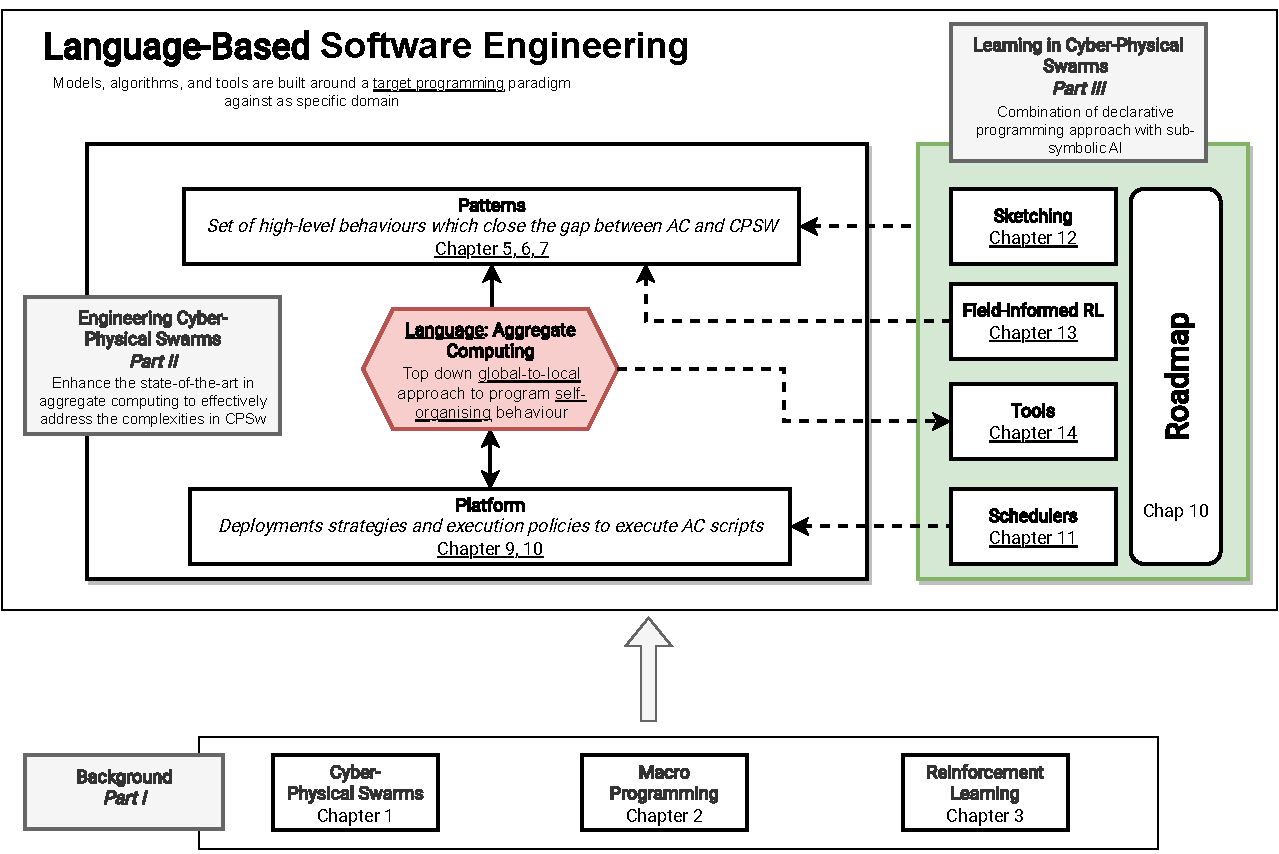
\includegraphics[width=\textwidth]{chapters/img/contribution-visual-2.drawio.pdf}
    \caption{Graphical overview of the thesis contributions.}\label{fig:contributions}
\end{figure}
\section{Thesis structure}
This thesis is organized as follows.
\Cref{chap:introduction} sets the stage by presenting an exhaustive overview of the research context, 
 elucidating the critical role of language-based engineering in complex systems. 
 This chapter also provides a roadmap of the thesis, enumerating its key contributions and thematic structure.

\Cref{part:background} lays the groundwork by delving into the theoretical pillars that sustain both standard and hybrid approaches in this domain. 
 It comprises \Cref{chap:cpsw}, which articulates the specific characteristics and challenges posed by \acp{cpsw}, and \Cref{chap:macro-programming}, 
 which offers an in-depth explanation of the aggregate computing paradigm and its associated programming model.
 Finally, \Cref{chap:marl} provides an exhaustive overview of the current landscape of reinforcement learning, 
 setting the stage for the terminologies and concepts deployed in subsequent chapters. 

\Cref{part:engineering} focuses on the practical engineering aspects pertaining to \acp{cpsw}. 
 It starts with \Cref{chap:eng:clustering}, introducing a groundbreaking algorithm designed for sensing-based clustering that has applications in collective decision-making. 
 Next, \Cref{chap:eng:decentralization} unveils a design pattern adept at encapsulating collective decision-making processes influenced by environmental variables. 
 \Cref{chap:eng:macroswarm} elaborates on a pioneering API for enabling coordinated movement and collective choices.
 Furthermore, \Cref{chap:eng:frp} presents an innovative programming model engineered specifically for \acp{cpsw}, aiming to enhance the efficiency of collective computations. 
 Finally, \Cref{chap:eng:multitier} expounds a contemporary deployment strategy that employs aggregate computing across the edge-cloud continuum.

\Cref{part:learning} focuses on contemporary hybrid learning methodologies applicable to \acp{cpsw}.  
 \Cref{chap:learning:roadmap} sketches a comprehensive roadmap for the amalgamation of aggregate computing and machine learning. 
 \Cref{chap:learning:sketching} introduces a groundbreaking technique for synthesizing collective programs. 
 In addition, \Cref{chap:rl:field-informed} presents an inventive approach to reinforcement learning within \acp{cpsw}, grounded in field calculus. 
 \Cref{chap:rl:schedulers} details a cutting-edge strategy for distributed scheduling in these complex systems. 
 Concluding this part, \Cref{chap:rl:scarlib} introduces an advanced toolkit designed for hybrid aggregate computing, 
 leveraging state-of-the-art deep learning libraries.

Finally, \Cref{chap:wrap-up} synthesizes the thesis contributions, drawing conclusions and laying out avenues for future research in this evolving field.

\printbibliography[title=Reference,heading=bibintoc]
\end{refsection}
\begin{refsection}
\section{Publication List}
\section*{2021}
\begin{enumerate}
    \item \fullcite{casadei2021programming}
    \item \fullcite{aguzzi2021scafi} 
    \item \fullcite{aguzzi2021research}
    \item \fullcite{aguzzi2021towards} \\ \textbf{Body of \Cref{chap:eng:multitier}}
    \item \fullcite{delnevo2021encouraging}
\end{enumerate}
\section*{2022}
\begin{enumerate}
    \item \fullcite{aguzzi2022towards} \\ \textbf{Body of \Cref{chap:learning:sketching}}
    \item \fullcite{casadei2022scafi} \\ \textbf{Body of \Cref{sec:scafi}}
    \item \fullcite{aguzzi2022dynamic} \\ \textbf{Body of \Cref{chap:eng:decentralization}}
    \item \fullcite{aguzzi2022addressing} \\ \textbf{Body of \Cref{chap:rl:schedulers}}
    \item \fullcite{aguzzi2022machine} \\ \textbf{Body of \Cref{chap:learning:roadmap}}
    \item \fullcite{casadei2022towards}
\end{enumerate}
\section*{2023}
\begin{enumerate}
    \item \fullcite{aguzzi2023field} \\ \textbf{Body of \Cref{chap:eng:clustering}}
    \item \fullcite{domini2023scarlib} \\ \textbf{Body of \Cref{chap:rl:scarlib}}
    \item \fullcite{aguzzi2023macroswarm} \\ \textbf{Body of \Cref{chap:eng:macroswarm}}
    \item \fullcite{aguzzi2023acgnn} \\ \textbf{Body of \Cref{chap:rl:field-informed}}
    \item \fullcite{aguzzi2023frasp} \\ \textbf{Body of \Cref{chap:eng:frp}}
    \item \fullcite{aguzzi2023tutorial} 
\end{enumerate}
\end{refsection}
